\documentclass[12pt,letterpaper]{article}
\usepackage{fullpage, lastpage, fancyhdr, enumerate}
\usepackage[top=2cm, bottom=4.5cm, left=2.5cm, right=2.5cm]{geometry}
\usepackage{amsmath,amsthm,amsfonts,amssymb,amscd}
\usepackage{mathrsfs, listings, hyperref, enotez}
\usepackage{xcolor, graphicx}
\usepackage[style=chicago-authordate,autocite=inline,backend=bibtex]{biblatex}
\graphicspath{{./images}}
\let\footnote=\endnote
\setenotez{list-name={Sources}}

\setlength{\parindent}{0.0in}
\setlength{\parskip}{0.05in}

\title{A Bayesian Approach to Hit Probability}
\author{Matthew Bernstein}

\addbibresource{bayes-hit-prob.bib}

\begin{document}

\maketitle

\section*{Introduction}
Expected Batting Average ($xBA$) is an attempt to quantify a hitter`s batting average using only the batted balls launch angle and exit velocity. Each batted ball is assigned an expected batting average based on how often comparable batted balls have become hits\footfullcite{mlb_expected_nodate}. This attempts to remove factors such as weather and defensive ability to isolate hitter skill and can be an important tool in assessing hitter ability.

The current xBA model is based solely on empirical data. This provides good predictive qualities but comes with some notable drawbacks. First, due to the reliance on historical data, access to that data is necessary to calculate it for future batted balls. This method also does not delineate between balls hit in different environments or different “eras”. The 2023 MLB season brought rule changes, notably banning the defensive shift, that could cause future batted balls to be hits while previous ones would not. Finally, Statcast only uses two elements of a batted ball for predictions. Other features, such as spray angle and distance, could improve predictive power. 

A model to determine the probability of any batted ball to be a hit would be a more accessible way to determine if the $xBA$ for a particular hitter. It could also be trained on specific subsets of data, such as from a specific park or time period, to focus the model for specific situations. 

\section*{Statcast Baseline}
The dataset includes all batted ball events from June 2022, with all sacrifice bunts, hits, and flyballs removed. In order to compare the model, a Statcast classification of every batted ball was calculated using the following formula:
\begin{align*}
    Hit =
        \begin{cases}
            1 & \text{if } xBA \ge 0.500\\
            0 & \text{if } xBA < 0.500
        \end{cases}
\end{align*}

The data was partitioned randomly into a training and test set on a 70/30 split. In addition to Statcast classifications, an additional control of predicting 0, or ``out", everytime was used as a reference. Table \ref{tab:baseline_acc} shows accuracy of the baseline methods.

\begin{table}[!htb]
    \centering
    \begin{tabular}{|r|c|c|c|c|}
        \hline
        & Accuracy & Sensitivity & Specificity & F1 Score \\ \hline
        Statcast & 0.800 & 0.607 & 0.895 & 0.667 \\ \hline
        Alaways Out & 0.671 & 0.0000 & 1.000 & 0.000 \\ \hline
    \end{tabular}
    \caption{Scores for baseline models}
    \label{tab:baseline_acc}
\end{table}

The Statcast classifications are quite accurate on the whole, but is worse at successfully predicting hits than outs. Since around 2/3 of all batted balls are outs, predicting a batted ball as an out should be the default classification.

\section*{Simple Bayesian Model}

First a bayesian logistic regression was fitted using the training data where $p$ is the probability that any batted ball is a hit
\begin{align*}
    log(\frac{p}{1-p}) = \beta_0 + \beta_1(\text{Launch Angle}) + \beta_2(\text{Exit Velocity})
\end{align*}
$\beta_i$ were given weakly informative priors
\begin{align*}
    \beta_0 &\sim \mathcal{N}(0, 2.5^2)\\
    \beta_1 &\sim \mathcal{N}(0, 10^2)\\
    \beta_2 &\sim \mathcal{N}(0, 10^2)
\end{align*}

\section*{Extended Bayesian Model}
Besides launch angle and exit velocity, there are other descriptive characteristics of batted balls, notably spray angle and distance. Spray angle defines the lateral angle of the batted ball. $0^{\circ}$ signifies directly up the middle, a negative angle is a pulled ball, regardless of batter handedness, and a positive angle is a ball hit to the opposite field. Spray angle was calculated from statcast data using Bill Pettis formula\footfullcite{petti_research_2017}. Hit distance is defined as how far the ball traveled before hitting the ground or being touched by a defender, the wall, or the stands\footfullcite{mlb_hit_nodate}. 

In addition, instead of directly using launch angle, this model separates batted balls into groups based on launch angle as defined by Statcast\footfullcite{mlb_launch_nodate}. Therefore each batted ball type has different coefficients, esentially creating 4 distinct models.
\begin{align*}
    log(\frac{p}{1-p}) &= \beta_0 + \beta_{0,i} + \beta_{1,i}(Exit Velocity) + \beta_{2,i}(\text{Spray Angle}) + \beta_{3,i}(\text{Hit Distance})\\
    i &\in \{GB, LD, FB, PU\}
\end{align*}
As with the simple bayes model, weakly informative priors were put on all coefficients.

\section*{Results}

Tables \ref{tab:simple_coef} and \ref{tab:ext_coef} detail the mean coefficients of the simple and extended bayesian regression respectively. Separating the group level effects shows how different types of batted balls should be treated differently. The coefficient for exit velocity in the simple model is positive, meaning increasing exit velocity increases the probability of being a hit. However, when breaking out the different batted ball types, both fly balls and pop ups have negative coefficients for exit velocity. This makes sense given that balls hit hard at high angles have longer hang times, meaning more time for defenders to track and catch. This effect can be seen as well in the negative coefficient for distance for line drives. Farther hit line drives are more likely to be caught as line drives that are hits often land between the infielders and the outfielders.

A negative coefficient for spray angle implies that pulled balls are more likely to be hits and a positive coefficient means a ball hit to the opposite side is more likely to be a hit. Grounders hit to the opposite side are more likely to be hits due to the prevalence of the shift. Hitting to the opposite side hits "against" the shift, where the defense is likley to leave holes.

\begin{table}[!htp]
    \centering
    \begin{tabular}{|r|c|c|c|}
        \hline
        & $\beta_0$ & $\beta_1$ (Launch Angle) & $\beta_2$ (Exit Velocity)\\ \hline
        Mean coefficient & -4.552 & -0.005 & 0.043 \\ \hline
    \end{tabular}
    \caption{Coefficients for simple bayes model}
    \label{tab:simple_coef}
\end{table}

\begin{table}[!htp]
    \centering
    \begin{tabular}{|r|c|c|c|c|}
        \hline
        & $\beta_0$ & $\beta_1$ (Exit Velocity) & $\beta_2$ (Spray Angle) & $\beta_3$ (Distance)\\ \hline
        Common      & -2.467 & & &\\ \hline
        Ground Ball & -0.649 & 0.019  & 0.025  & 0.015\\ \hline
        Line Drive  & 0.840  & 0.041  & -0.005 & -0.007\\ \hline
        Fly Ball    & -0.107 & -0.082 & -0.025 & 0.028\\ \hline
        Pop Up      & -1.059 & -0.069 & 0.022  & 0.027\\ \hline
    \end{tabular}
    \caption{Coefficients for extended bayes model}
    \label{tab:ext_coef}
\end{table}

Figure \ref{fig:results_roc} displays the ROC of the statcast baseline, using $xBA$ as the prediction scores, as well as the two bayesian regressions. Table \ref{tab:results_acc} compares various accuracy metrics for the models. The Simple Bayes model performs poorly compared to the Statcast classifications. Specifically, the Simple Bayes model misclassifies almost all the hits as outs. Due to the imbalance of hits versus outs, this does not impact the accuracy as much which is why sensitivity or F1 score are better metrics for model evaluation for this data. The Extended Bayes model performs very similarly to the Statcast classifier, with a slightly higher sensitivity at the cost of a slightly lower specificity. While the regression cannot capture the nuances that historical data can, the added data makes up most of that gap. 

\begin{figure}[!htb]
    \centering
    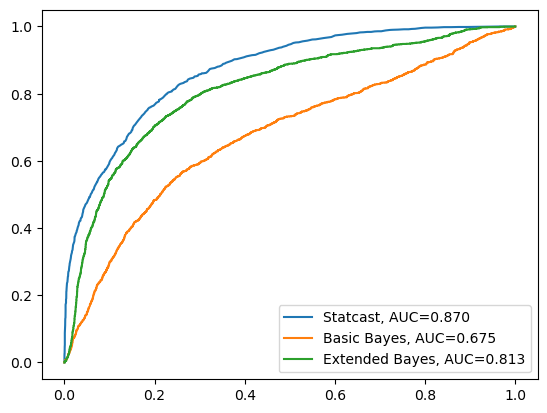
\includegraphics[width=0.5\textwidth]{all_roc}
    \caption{ROC curve of all methods}
    \label{fig:results_roc}
\end{figure}

\begin{table}[!htb]
    \centering
    \begin{tabular}{|r|c|c|c|c|}
        \hline
        & Accuracy & Sensitivity & Specificity & F1 Score \\ \hline
        Statcast & 0.800 & 0.607 & 0.895 & 0.667 \\ \hline
        Simple Bayes & 0.684 & 0.102 & 0.970 & 0.176 \\ \hline
        Extended Bayes & 0.779 & 0.610 & 0.862 & 0.645 \\ \hline
    \end{tabular}
    \caption{Scores for all models}
    \label{tab:results_acc}
\end{table}

\section*{Conclusion}

Statcast's $xBA$ model provides excellent insight into a hitters skill based on what the hitter can control. However, it's reliance on empirical data and opaque methodology make it less accesible for deeper insight. A well trained model can both provide customization from the training data as well as include more of the information available. The model performed almost as well as using the Statcast $xBA$ as a classifier. It had slighly improved sensitivity at the cost of slightly reduced overall accuracy. This demonstrates that it could be a suitable replacement as for hit probability.

\section*{Future Work}

Weakly informative priors were used for all coefficients while training this model. Further research could be done to find better priors fo the coefficients. In addition, the training data for this model was from all environments, further investigation should be done to see if the model would perform better on data from specific ballparks. Finally, adjustments to the spray angle formula as well as further segregating batted ball types into more categories, such as high and low line drives, coud improve classification.

\noindent\rule{\textwidth}{1pt}
\printendnotes

\end{document}